\section{Introdução}

Em meio a diversas hipóteses sobre o surgimento da Terra e a evolução genômica
foram abertas a um longo período de discussão e debate que nos rodeia até hoje trazendo teorias de diferentes campos com intenção de esclarecer todo esse passado apagado. Uma teoria bem popular é a Panspermia cósmica [1]\citep{1}. 

Para ter uma ideia sobre a evolução molecular, modelos biológicos [17,18]\citep{17,18}  e
matemáticos [19]\citep{19} foram desenvolvidos. Na área de matemática, o modelo mais conhecido é o Modelo de Eigen [5,6]\citep{5,6} que descreve a evolução do fago QB por equações diferenciais. Na área biológica suposição do \emph{“Mundo de RNA”} [7]\citep{7} se tornando muito visado por trazer a descoberta sobre RNA catalítico [8,9]\citep{8,9}. Com esse ganho de conhecimento e popularidade foi um enorme passo entre a junção da biologia e tecnologia proporcionando o sequenciamento e o PCR (polymerase chain reaction) [10]\citep{10} com ciclos de AMS (amplificação mutação e seleção) [11]\citep{11}, assim, podendo proporcionar diversos estudos e pesquisas na área de biotecnologia. O modelo de AMS que teve a intenção de ser mimetizado nessa pesquisa foi SELEX \emph{(systematic evolution of ligands by exponential enrichment)} [12,13]\citep{12,13}, um sistema usado no tratamento ou detecção de doenças[14,15,16]\citep{14,15,16}.

\subsection{Teoria da informação e evolução molecular}
A teoria da informação [4]\citep{4} está tão presente no dia a dia, é a área que trabalha com símbolos, mensagens e canais, seu feito é em diversas áreas do conhecimento.
Desenvolvida em 1948 por Shannon. O princípio básico da teoria da informação é estudar a transmissão de dados, onde, os símbolos podem ser considerados dados ou mensagens, o canal seria o meio ou fio onde seria feito o envio e recepção da mensagem. Como esse canal não é perfeito, pode haver interferências que atrapalhem no envio desses símbolos fazendo com que alguns deles sem percam no caminho. Quando aplicamos esse mesmo princípio na Biologia, as mensagens passam a serem os nucleotídeos ou aminoácidos, o canal seria a replicação pois é o momento onde acontece a transcrição e os erros mimetizam o processo de mutação.

\subsection{Selex}
Se baseando no estudo da evolução do RNA catalítico in vitro, Joyce desenvolveu um
protocolo que trabalhavam com ciclos de amplificação, mutação e seleção [11]\citep{11}. No ano seguinte, Ellington e Szostak [12]\citep{12} e Tuerk e Gold [13]\citep{13} desenvolveram o SELEX
(systematic evolution of ligands by exponential enrichment) [12,13]\citep{12,13}. Um sistema onde os alvos buscam moléculas aptas ao seu interesse fazendo esse processo por diversos ciclos, se baseando em etapas de amplificação, mutação e seleção.

\subsection{Entropia}

Para a análise da grande massa de moléculas foi necessária uma ferramenta
desenvolvida por Shannon em 1948 [3]\citep{3} chamada entropia de Shannon [4]\citep{4}, com ela foi
possível medir o grau de desordem entre cada índice das moléculas. A equação da entropia de
Shannon (\ref{entropia-shannon}) é dada pela seguinte expressão:

\begin{equation}
    \label{entropia-shannon}
    \mathbf{H(x) = -\sum\limits_{i=1}^{n}p(x_i)log p(x_i)}
\end{equation}

$$p(x_i)=\text{probabilidade de ocorrer } x_i\text{ em X.}$$

Para calcular a entropia nas moléculas, foi feito por índice de base assim cada
coluna tinha o seu valor de entropia calculado e logos após tirando a média dessas
entropias, segue abaixo a figura \ref{fig:example-entropia} sobre o desenvolvimento da entropia:

\begin{figure}[!h]
    \centering
    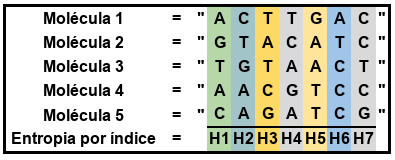
\includegraphics[scale=0.7]{figures/img-entropia.png}
    \caption{Desenvolvimento da entropia}
    \label{fig:example-entropia}
\end{figure}